\documentclass[a4paper,fleqn]{cas-sc}

\usepackage[numbers]{natbib}
\usepackage{amsmath,amssymb,amsfonts}
\usepackage{booktabs}
\usepackage{graphicx}
\usepackage{hyperref}
\usepackage{tabularx}
\usepackage{multirow}
\usepackage{microtype}
\usepackage{lastpage}

% Khắc phục lỗi "Page 13 of 12" của template Elsevier cas-sc:
% Macro \lastpage mặc định ghi ra .aux trước khi trang cuối shipout, dẫn tới sai tổng số trang.
% Ghi đè \lastpage bằng nhãn chuẩn từ gói lastpage:
\AtBeginDocument{%
  \def\lastpage{\pageref*{LastPage}}%
}

\begin{document}
\let\WriteBookmarks\relax
\def\floatpagepagefraction{1}
\def\textpagefraction{.001}

% Tiêu đề ngắn ở đầu trang
\shorttitle{Exact SAT-Based Solving for the N-Queens Problem}
\shortauthors{Hoang Lam Tung}

% Tiêu đề chính
\title [mode = title]{Exact Solving Approaches for the N-Queens Problem: A Comparative Study of SAT Cardinality Encodings, Constraint Programming, and Integer Linear Programming}

% Tác giả & Đơn vị công tác
\author[1]{Hoang Lam Tung}[orcid=]
\cormark[cor1]
\ead{24021661@vnu.edu.vn}

\address[1]{Faculty of Information Technology, VNU University of Engineering and Technology, 144 Xuan Thuy, Cau Giay, Hanoi, Vietnam}

\cortext[cor1]{Corresponding author}

% ==================== ABSTRACT ====================
\begin{abstract}
The $N$-Queens problem is a classic combinatorial benchmark widely used to evaluate exact search algorithms and constraint reasoning engines. In this study, we investigate exact solving paradigms for $N$-Queens, focusing on Boolean Satisfiability (SAT) formulations using modern cardinality encodings. Specifically, we examine multiple At-Most-One (AMO) encoding techniques—including Pairwise, Sequential Counter, Commander, Product, and Binary encodings—implemented via the PySAT framework \cite{ignatiev2018pysat}. We benchmark state-of-the-art CDCL SAT solvers (CaDiCaL, Glucose, Kissat) against leading commercial and open-source exact solvers across Constraint Programming (IBM ILOG CPLEX CP, Google OR-Tools CP-SAT) and Mixed-Integer Linear Programming (Gurobi, CPLEX MIP). Extensive computational experiments on large board sizes ($N$ up to 1000) demonstrate that linear-size cardinality encodings significantly alleviate clause explosion, allowing SAT solvers and CP-SAT to substantially outperform traditional MIP formulations in scalability and solving efficiency. While MIP solvers encounter severe performance degradation and timeout ($>300$\,s) for $N \ge 256$, OR-Tools CP-SAT and PySAT with CaDiCaL successfully solve $N = 1000$ in just $28.6$\,s and $78.2$\,s, respectively.
\end{abstract}

\begin{keywords}
N-Queens problem \sep SAT solving \sep Cardinality constraints \sep PySAT \sep Constraint Programming \sep Integer Linear Programming
\end{keywords}

\maketitle

% ==================== 1. INTRODUCTION ====================
\section{Introduction}
\label{sec:intro}

The $N$-Queens problem is a classic benchmark in artificial intelligence and discrete combinatorial optimization. Formulated as placing $N$ non-attacking queens on an $N \times N$ chessboard, it serves as a canonical model for Constraint Satisfaction Problems (CSPs). Two queens attack each other if they share the same row, column, or diagonal; thus, a valid configuration requires placing exactly $N$ queens such that no two queens attack each other.

While heuristic and local search algorithms (such as min-conflicts \cite{minton1992solving}) can quickly find a single solution for large boards, exact solving paradigms remain essential for certifying unsatisfiability, enumerating solutions, and systematically evaluating constraint reasoning engines. In practice, three main exact paradigms are commonly used:
\begin{enumerate}
    \item \textbf{Constraint Programming (CP):} Models problems using integer variables and global constraints like \texttt{AllDifferent} \cite{ibm2022cplex,regin1994filtering}.
    \item \textbf{Mixed-Integer Linear Programming (MIP):} Formulates conditions as linear inequalities over binary variables, solved via branch-and-cut (e.g., Gurobi \cite{gurobi2025}, CPLEX \cite{ibm2022cplex}).
    \item \textbf{Boolean Satisfiability (SAT):} Translates constraints into Conjunctive Normal Form (CNF) solved by Conflict-Driven Clause Learning (CDCL) engines (e.g., CaDiCaL, Glucose, Kissat) \cite{biere2021handbook}.
\end{enumerate}

Despite the efficiency of modern CDCL SAT solvers, translating high-level constraints into CNF faces a major challenge known as \textit{clause explosion}. An $N \times N$ chessboard contains $4N - 2$ diagonals. A naive Pairwise encoding across rows, columns, and diagonals generates $\Theta(N^3)$ clauses \cite{prestwich2009cnf}, causing memory exhaustion for $N \ge 256$. To overcome this limitation, advanced cardinality encodings—such as Sequential Counter \cite{sinz2005towards}, Commander \cite{klieber2007commander}, Product \cite{chen2010new}, and Binary \cite{frisch2005symmetry} encodings—reduce clause counts to linear bounds $\mathcal{O}(m)$ by introducing auxiliary variables.

In this work, we present a comparative study of exact solving approaches for $N$-Queens, focusing on SAT cardinality encodings in the PySAT framework \cite{ignatiev2018pysat}. The main contributions of this paper are:
\begin{itemize}
    \item We formulate and evaluate five At-Most-One (AMO) encodings (Pairwise, Sequential Counter, Commander, Product, Binary) for $N$-Queens using PySAT.
    \item We benchmark CDCL SAT solvers (CaDiCaL, Glucose, Kissat) across board sizes up to $N = 1000$.
    \item We conduct a cross-paradigm comparison against Constraint Programming (CPLEX CP, Google OR-Tools CP-SAT) and Mixed-Integer Programming (Gurobi, CPLEX MIP).
    \item We provide an open-source, reproducible repository containing all benchmark implementations.
\end{itemize}

The rest of this paper is organized as follows. Section~\ref{sec:background} presents the mathematical models for CP and MIP. Section~\ref{sec:sat_encodings} details the SAT formulation and cardinality encodings. Section~\ref{sec:experiments} reports empirical results and discussion. Section~\ref{sec:conclusion} concludes the paper.

% ==================== 2. BACKGROUND ====================
\section{Background and Problem Formulations}
\label{sec:background}

\subsection{Formal Problem Definition as a CSP}
\label{subsec:csp_definition}
The $N$-Queens problem requires placing $N$ mutually non-attacking chess queens on an $N \times N$ chessboard. Formally, it can be framed as a canonical Constraint Satisfaction Problem (CSP) defined by the triplet $\langle X, D, C \rangle$:
\begin{itemize}
    \item \textbf{Variables:} $X = \{Q_1, Q_2, \dots, Q_N\}$, where variable $Q_i$ represents the position of the queen situated in row $i \in \{1, \dots, N\}$.
    \item \textbf{Domains:} $D = \{D_1, D_2, \dots, D_N\}$, where each domain $D_i = \{1, 2, \dots, N\}$ designates the candidate column coordinates available for row $i$.
    \item \textbf{Constraints:} $C = \{C_{\text{col}}, C_{\text{diag\_maj}}, C_{\text{diag\_min}}\}$, prohibiting distinct queens from sharing columns or diagonals.
\end{itemize}

By associating exactly one variable with each row, row-level conflicts are eliminated by construction, reducing the unconstrained state space from $\binom{N^2}{N}$ arbitrary board configurations down to $N^N$. For any pair of distinct queens $(Q_{i_1}, Q_{i_2})$ with $1 \le i_1 < i_2 \le N$, the non-attacking requirements are formalized as:
\begin{enumerate}
    \item \textbf{Column non-conflict:} No two queens occupy the same column:
    \begin{equation}
        Q_{i_1} \ne Q_{i_2}, \quad \forall 1 \le i_1 < i_2 \le N \label{eq:cond_col}
    \end{equation}
    Constraint~(\ref{eq:cond_col}) guarantees that any valid queen placement corresponds to a permutation of the column set $\{1, \dots, N\}$, shrinking the effective candidate space to $N!$.
    \item \textbf{Major diagonal non-conflict:} Queens cannot share diagonals of slope $+1$ ($j - i = \text{const}$):
    \begin{equation}
        Q_{i_1} - i_1 \ne Q_{i_2} - i_2, \quad \forall 1 \le i_1 < i_2 \le N \label{eq:cond_diag_maj}
    \end{equation}
    \item \textbf{Minor diagonal non-conflict:} Queens cannot share diagonals of slope $-1$ ($i + j = \text{const}$):
    \begin{equation}
        Q_{i_1} + i_1 \ne Q_{i_2} + i_2, \quad \forall 1 \le i_1 < i_2 \le N \label{eq:cond_diag_min}
    \end{equation}
\end{enumerate}

\subsection{Constraint Programming (CP) Formulation}
\label{subsec:cp_formulation}
In Constraint Programming, global constraints provide high-level declarative abstractions backed by specialized polynomial-time propagation algorithms. The $N$-Queens problem is modeled using three \texttt{AllDifferent} constraints applied over linear shifts of the row variables $Q_i$:
\begin{align}
    \text{AllDifferent}(Q_1, Q_2, \dots, Q_N) \label{eq:cp_col} \\
    \text{AllDifferent}(Q_1 - 1, Q_2 - 2, \dots, Q_N - N) \label{eq:cp_diag1} \\
    \text{AllDifferent}(Q_1 + 1, Q_2 + 2, \dots, Q_N + N) \label{eq:cp_diag2}
\end{align}

\paragraph{Filtering and Inference Mechanics:}
Constraint~(\ref{eq:cp_col}) prevents column collisions, while Constraints~(\ref{eq:cp_diag1}) and~(\ref{eq:cp_diag2}) enforce diagonal independence via linear coordinate translations. In classical CP solvers (such as IBM ILOG CPLEX CP Optimizer \cite{ibm2022cplex}), \texttt{AllDifferent} constraints are propagated using Régin's bipartite matching algorithm \cite{regin1994filtering}. The algorithm builds a bipartite value graph $G = (X \cup V, E)$, computing maximum matchings via the Hopcroft-Karp algorithm and strongly connected components (SCCs) via Tarjan's algorithm. This achieves Generalized Arc Consistency (GAC) in $\mathcal{O}(N^{1.5} \cdot |D|)$ time, pruning inconsistent values from variable domains prior to search branching.

In modern hybrid solvers like Google OR-Tools CP-SAT, global constraints are paired with Lazy Clause Generation (LCG). Rather than executing domain filtering in isolation, CP-SAT lazily maps integer domain prunings into clausal explanations that feed a core Conflict-Driven Clause Learning (CDCL) engine. This combines the high-level pruning power of CP with the conflict-directed backjumping and nogood recording of SAT solvers.

\subsection{Mixed-Integer Linear Programming (MIP) Formulation}
\label{subsec:mip_formulation}
The MIP formulation models the chessboard using an $N \times N$ binary decision matrix $X \in \{0, 1\}^{N \times N}$, where binary variable $x_{i,j} = 1$ if a queen is placed at cell $(i, j)$, and $x_{i,j} = 0$ otherwise. Because $N$-Queens is a feasibility problem, the objective function is arbitrary and set to minimize zero:
\begin{align}
    \min \quad & 0 \label{eq:ilp_obj} \\
    \text{s.t.} \quad & \sum_{j=1}^{N} x_{i,j} = 1, \quad \forall i \in \{1, \dots, N\} \label{eq:ilp_row} \\
    & \sum_{i=1}^{N} x_{i,j} = 1, \quad \forall j \in \{1, \dots, N\} \label{eq:ilp_col} \\
    & \sum_{\substack{1 \le i, j \le N \\ j - i = k}} x_{i,j} \le 1, \quad \forall k \in \{-(N-2), \dots, N-2\} \label{eq:ilp_diag1} \\
    & \sum_{\substack{1 \le i, j \le N \\ i + j = k}} x_{i,j} \le 1, \quad \forall k \in \{3, \dots, 2N-1\} \label{eq:ilp_diag2} \\
    & x_{i,j} \in \{0, 1\}, \quad \forall i, j \in \{1, \dots, N\} \label{eq:ilp_var}
\end{align}
Equations~(\ref{eq:ilp_row}) and~(\ref{eq:ilp_col}) mandate exactly one queen per row and column. Inequalities~(\ref{eq:ilp_diag1}) and~(\ref{eq:ilp_diag2}) enforce at most one queen on every major and minor diagonal of length $\ge 2$. In total, the formulation specifies $N^2$ binary variables and $2N + (2N - 3) + (2N - 3) = 6N - 6$ linear constraints.

\paragraph{Theoretical Cause of MIP Inefficiency on Large $N$:}
Although the MIP formulation has only $\mathcal{O}(N)$ constraints, commercial branch-and-cut solvers (such as Gurobi \cite{gurobi2025} and CPLEX MIP \cite{ibm2022cplex}) experience severe performance degradation and timeout ($> 300$\,s) for $N \ge 256$. This failure originates from three fundamental structural weaknesses of the continuous Linear Programming (LP) relaxation ($0 \le x_{i,j} \le 1$):
\begin{enumerate}
    \item \textbf{Trivial Uniform Fractional Solution:} The uniform assignment $x_{i,j}^* = 1/N$ for all $1 \le i, j \le N$ satisfies every constraint: $\sum_{j=1}^N (1/N) = 1$ for all rows, $\sum_{i=1}^N (1/N) = 1$ for all columns, and for any diagonal of length $L \le N$, $\sum (1/N) = L/N \le 1$.
    \item \textbf{Total Absence of Objective Guidance:} Because the objective function is $\min 0$, the uniform fractional point $x_{i,j}^* = 1/N$ achieves an optimal LP objective value of 0. Dual simplex iterations yield identical lower bounds across all search nodes, providing zero gradient guidance for variable selection.
    \item \textbf{Inefficacy of Polyhedral Cuts:} Standard cutting planes (Gomory cuts, clique cuts) cannot tighten the fractional polytope effectively due to high permutation symmetry, reducing branch-and-bound to an exhaustive enumeration over a $2^{N^2}$ search tree.
\end{enumerate}

\subsection{Cross-Paradigm Comparison}
\label{subsec:paradigm_comparison}
Table~\ref{tab:paradigm_comparison} summarizes the three exact paradigms across decision variable representations, constraint counts, inference mechanisms, and primary scalability bottlenecks.

\begin{table}[ht]
\centering
\caption{Systematic comparison of exact modeling paradigms for the $N$-Queens problem.}
\label{tab:paradigm_comparison}
\begin{tabularx}{\linewidth}{lXXXX}
\toprule
\textbf{Paradigm} & \textbf{Decision Variables} & \textbf{Constraint System} & \textbf{Core Inference Engine} & \textbf{Primary Bottleneck} \\
\midrule
Constraint Programming (CP) & $N$ integers ($D_i = \{1, \dots, N\}$) & 3 global \texttt{AllDifferent} constraints & Bipartite matching (GAC) + Lazy Clause Generation & Tree-search thrashing without nogood learning \\
Mixed-Integer Programming (MIP) & $N^2$ binary variables ($x_{i,j} \in \{0, 1\}$) & $6N - 6$ linear equations \& inequalities & Simplex LP relaxation + Branch-and-Cut & Flat LP relaxation ($x_{i,j} = 1/N$), zero dual bound signal \\
Boolean Satisfiability (SAT) & $N^2$ primary $+ \mathcal{O}(N)$ auxiliary Booleans & CNF clauses ($\mathcal{O}(N)$ to $\mathcal{O}(N^3)$) & CDCL: 2WL unit propagation + 1-UIP conflict analysis & Clause explosion if naive pairwise encoding is used \\
\bottomrule
\end{tabularx}
\end{table}

% ==================== 3. SAT-BASED ENCODING ====================
\section{SAT-Based Formulations and Cardinality Encodings}
\label{sec:sat_encodings}

\subsection{Boolean Variables and Coordinate Mapping}
\label{subsec:sat_decomposition}

\subsubsection{Decision Variables and DIMACS Index Mapping}
The $N \times N$ chessboard is modeled using $N^2$ Boolean decision variables $B_{i,j} \in \{\text{True}, \text{False}\}$ for $1 \le i, j \le N$, where $B_{i,j} = \text{True}$ indicates that a queen is positioned at row $i$ and column $j$.

In standard DIMACS CNF format, literals are identified by non-zero integers. The 2D grid coordinate $(i, j)$ is mapped onto a unique 1D integer identifier $\text{id}(i, j) \in \{1, \dots, N^2\}$ using row-major linearization:
\begin{equation}
    \text{id}(i, j) = (i - 1) \cdot N + j, \quad \forall i, j \in \{1, \dots, N\} \label{eq:dimacs_mapping}
\end{equation}
Conversely, any DIMACS literal index $v \in \{1, \dots, N^2\}$ maps back to chessboard coordinates via:
\begin{equation}
    i = \left\lfloor \frac{v - 1}{N} \right\rfloor + 1, \qquad j = ((v - 1) \bmod N) + 1 \label{eq:dimacs_inverse}
\end{equation}

\subsubsection{Diagonal Coordinate Indexing}
An $N \times N$ chessboard contains $2N - 1$ major diagonals and $2N - 1$ minor diagonals. Diagonals of length 1 (located at the 4 board corners) can accommodate at most one queen by definition and impose no non-trivial constraints. Therefore, cardinality constraints are posted exclusively over the $2N - 3$ non-trivial diagonals of length $\ge 2$:
\begin{itemize}
    \item \textbf{Major Diagonals ($j - i = k$):} Parameterized by offset $k \in \{-(N-2), \dots, N-2\}$, the variable set $D_k^{\text{maj}}$ is defined as:
    \begin{equation}
        D_k^{\text{maj}} = \left\{ B_{i, i+k} \;\middle|\; \max(1, 1-k) \le i \le \min(N, N-k) \right\} \label{eq:diag_maj_set}
    \end{equation}
    \item \textbf{Minor Diagonals ($i + j = k$):} Parameterized by sum index $k \in \{3, \dots, 2N-1\}$, the variable set $D_k^{\text{min}}$ is defined as:
    \begin{equation}
        D_k^{\text{min}} = \left\{ B_{i, k-i} \;\middle|\; \max(1, k-N) \le i \le \min(N, k-1) \right\} \label{eq:diag_min_set}
    \end{equation}
\end{itemize}

\subsection{Decomposition into Cardinality Constraints}
\label{subsec:cardinality_decomposition}
For any non-empty subset of Boolean variables $S = \{v_1, v_2, \dots, v_m\}$, cardinality constraints constrain the number of assigned True literals:
\begin{itemize}
    \item \textbf{At-Least-One (ALO):} $\sum_{k=1}^m v_k \ge 1$ (at least one queen placed).
    \item \textbf{At-Most-One (AMO):} $\sum_{k=1}^m v_k \le 1$ (at most one queen placed).
    \item \textbf{Exactly-One (EO):} $\sum_{k=1}^m v_k = 1$, which decomposes logically as:
    \begin{equation}
        \text{EO}(S) \iff \text{ALO}(S) \wedge \text{AMO}(S)
    \end{equation}
\end{itemize}

The global CNF formula $\mathcal{F}_{N\text{-Queens}}$ is the conjunction of four structural constraint sets:
\begin{equation}
    \mathcal{F}_{N\text{-Queens}} = \mathcal{F}_{\text{rows}} \wedge \mathcal{F}_{\text{cols}} \wedge \mathcal{F}_{\text{diag\_maj}} \wedge \mathcal{F}_{\text{diag\_min}}
\end{equation}
Table~\ref{tab:sat_decomposition_summary} summarizes the cardinality types and cardinality counts across all subsets.

\begin{table}[ht]
\centering
\caption{Summary of constraint subsets and cardinality types in the SAT decomposition.}
\label{tab:sat_decomposition_summary}
\begin{tabular}{llrr}
\toprule
\textbf{Constraint Category} & \textbf{Cardinality Type} & \textbf{Number of Subsets} & \textbf{Subset Variable Count} \\
\midrule
Rows & Exactly-One ($\text{ALO} \wedge \text{AMO}$) & $N$ & $N$ \\
Columns & Exactly-One ($\text{ALO} \wedge \text{AMO}$) & $N$ & $N$ \\
Major Diagonals ($\ge 2$) & At-Most-One ($\text{AMO}$) & $2N - 3$ & $2 \le |D_k^{\text{maj}}| \le N$ \\
Minor Diagonals ($\ge 2$) & At-Most-One ($\text{AMO}$) & $2N - 3$ & $2 \le |D_k^{\text{min}}| \le N$ \\
\bottomrule
\end{tabular}
\end{table}

\subsection{At-Least-One (ALO) Encoding}
\label{subsec:alo_encoding}
The At-Least-One constraint $\sum_{k=1}^m v_k \ge 1$ maps directly to a single disjunctive clause containing all participating literals:
\begin{equation}
    \mathcal{F}_{\text{ALO}}(S) = \left( \bigvee_{k=1}^{m} v_k \right) = (v_1 \vee v_2 \vee \dots \vee v_m)
\end{equation}
For $N$-Queens, ALO constraints are posted exclusively on rows and columns:
\begin{align}
    \mathcal{F}_{\text{ALO}}^{\text{row}}(i) &= \bigvee_{j=1}^{N} B_{i,j}, \quad \forall i \in \{1, \dots, N\} \label{eq:alo_row} \\
    \mathcal{F}_{\text{ALO}}^{\text{col}}(j) &= \bigvee_{i=1}^{N} B_{i,j}, \quad \forall j \in \{1, \dots, N\} \label{eq:alo_col}
\end{align}
Equations~(\ref{eq:alo_row}) and~(\ref{eq:alo_col}) generate exactly $2N$ clauses without requiring auxiliary variables. Diagonal constraints omit ALO because an $N \times N$ board contains $4N - 6$ non-trivial diagonals but only $N$ queens, meaning the vast majority of diagonals must remain empty.

\subsection{At-Most-One (AMO) Cardinality Encodings}
\label{subsec:amo_encodings}
The At-Most-One constraint $\sum_{k=1}^m v_k \le 1$ represents the primary combinatorial challenge. On an $N \times N$ board, encoding AMO naively across rows, columns, and diagonals causes cubic clause explosion $\Theta(N^3)$, exhausting memory for $N \ge 256$. Below, we detail the mathematical formulations, intuitions, and complexity profiles of the five AMO encoding schemes implemented in this study.

\subsubsection{Pairwise (Direct) Encoding}
\paragraph{Intuition:} Forbids every pair of distinct variables in $S = \{v_1, \dots, v_m\}$ from being simultaneously True ($\neg(v_p \wedge v_q) \equiv \neg v_p \vee \neg v_q$).
\paragraph{CNF Formulation:}
\begin{equation}
    \mathcal{F}_{\text{AMO}}^{\text{pair}}(S) = \bigwedge_{1 \le p < q \le m} (\neg v_p \vee \neg v_q) \label{eq:amo_pairwise}
\end{equation}
\paragraph{Properties:}
\begin{itemize}
    \item \textbf{Auxiliary Variables:} $0$.
    \item \textbf{Clause Count:} $\binom{m}{2} = \frac{m(m-1)}{2} = \Theta(m^2)$.
    \item \textbf{Propagation:} Preserves Generalized Arc Consistency (GAC) through standard Unit Propagation (UP): as soon as one variable $v_p$ becomes True, UP immediately sets every other $v_q = \text{False}$ in $\mathcal{O}(1)$ time per clause.
    \item \textbf{Bottleneck:} For $N$-Queens, summing $\binom{|D_k|}{2}$ across all rows, columns, and diagonals produces $\approx \frac{7}{3} N^3$ clauses. For $N = 256$, this exceeds 16 million clauses, and for $N = 1000$, it requires $>2.3$ billion clauses, causing immediate out-of-memory (OOM) failures during CNF generation.
\end{itemize}

\subsubsection{Sequential Counter Encoding}
\paragraph{Intuition:} Proposed by Sinz \cite{sinz2005towards}, this encoding simulates a unary accumulator register using $m - 1$ auxiliary variables $s_1, \dots, s_{m-1}$. Variable $s_i = \text{True}$ signifies that \textit{at least one} variable in the prefix $\{v_1, \dots, v_i\}$ has been assigned True.
\paragraph{CNF Formulation:}
\begin{align}
    & (\neg v_1 \vee s_1) \label{eq:seq_init} \\
    & (\neg s_i \vee s_{i+1}), \quad && \forall 1 \le i \le m-2 \label{eq:seq_shift} \\
    & (\neg v_{i+1} \vee \neg s_i), \quad && \forall 1 \le i \le m-1 \label{eq:seq_conflict} \\
    & (\neg v_{i+1} \vee s_{i+1}), \quad && \forall 1 \le i \le m-2 \label{eq:seq_update}
\end{align}
\paragraph{Explanation of Clauses:}
\begin{itemize}
    \item Eq.~(\ref{eq:seq_init}) initializes the accumulator: if $v_1$ is True, $s_1$ must be True.
    \item Eq.~(\ref{eq:seq_shift}) enforces monotonic propagation: once the accumulator turns True at position $i$, it remains True for all subsequent positions $i+1, \dots, m-1$.
    \item Eq.~(\ref{eq:seq_conflict}) enforces the AMO invariant: if the prefix accumulator $s_i$ is already True, the subsequent candidate variable $v_{i+1}$ cannot be True.
    \item Eq.~(\ref{eq:seq_update}) updates the accumulator: if $v_{i+1}$ is True, the register at $i+1$ is activated.
\end{itemize}
\paragraph{Properties:}
\begin{itemize}
    \item \textbf{Auxiliary Variables:} $m - 1 = \Theta(m)$.
    \item \textbf{Clause Count:} Exactly $3m - 4 = \Theta(m)$ binary clauses (length 2).
    \item \textbf{Propagation:} Enforces GAC under Unit Propagation. When $v_k = \text{True}$, Eq.~(\ref{eq:seq_update}) sets $s_k = \text{True}$, Eq.~(\ref{eq:seq_shift}) propagates True to all $s_{k+1}, \dots, s_{m-1}$, and Eq.~(\ref{eq:seq_conflict}) drives all subsequent variables $v_{k+1}, \dots, v_m$ to False via UP.
\end{itemize}

\subsubsection{Commander Encoding}
\paragraph{Intuition:} Introduced by Klieber and Kwon \cite{klieber2007commander}, this divide-and-conquer technique partitions the $m$ literals into disjoint groups $G_1, G_2, \dots, G_g$, typically of size $k = 3$. Each group $G_r$ elects an auxiliary ``commander'' variable $c_r \in \{\text{True}, \text{False}\}$, which is True if and only if a literal in $G_r$ is True.
\paragraph{CNF Formulation:}
\begin{enumerate}
    \item \textbf{Intra-Group AMO:} At most one variable is True within each group $G_r$:
    \begin{equation}
        \bigwedge_{\substack{v_a, v_b \in G_r \\ a < b}} (\neg v_a \vee \neg v_b), \quad \forall r \in \{1, \dots, g\} \label{eq:cmd_intra}
    \end{equation}
    \item \textbf{Commander Linking:} The commander $c_r$ reflects the group state:
    \begin{align}
        & (\neg v \vee c_r), \quad \forall v \in G_r, \quad \forall r \in \{1, \dots, g\} \label{eq:cmd_link1} \\
        & \left( \neg c_r \vee \bigvee_{v \in G_r} v \right), \quad \forall r \in \{1, \dots, g\} \label{eq:cmd_link2}
    \end{align}
    \item \textbf{Inter-Group AMO:} At most one commander can be True across all groups:
    \begin{equation}
        \text{AMO}(c_1, c_2, \dots, c_g) \label{eq:cmd_inter}
    \end{equation}
    If $g > k$, Constraint~(\ref{eq:cmd_inter}) is applied recursively until a single root commander remains.
\end{enumerate}
\paragraph{Properties:}
\begin{itemize}
    \item \textbf{Auxiliary Variables:} $\approx \frac{m}{k - 1} = \Theta(m)$ for group size $k = 3$.
    \item \textbf{Clause Count:} $\approx 3.5m = \Theta(m)$, with maximum clause length $k + 1 = 4$.
    \item \textbf{Propagation:} Preserves GAC through UP across hierarchical levels.
\end{itemize}

\subsubsection{Product (2D Grid) Encoding}
\paragraph{Intuition:} Proposed by Chen \cite{chen2010new}, this method maps the $m$ literals onto a two-dimensional grid of dimension $p \times q$ such that $p \cdot q \ge m$. Optimal auxiliary variable efficiency is achieved by selecting $p = \lceil \sqrt{m} \rceil$ and $q = \lceil m / p \rceil \approx \sqrt{m}$. Each variable $v_k$ is indexed by a unique coordinate pair $(r, c)$. We define $p$ row selector variables $u_1, \dots, u_p$ and $q$ column selector variables $w_1, \dots, w_q$.
\paragraph{CNF Formulation:}
A variable $v_k$ at coordinate $(r, c)$ can be True only if both its row selector $u_r$ and column selector $w_c$ are True ($v_k \implies u_r \wedge w_c$):
\begin{align}
    & (\neg v_k \vee u_r) \wedge (\neg v_k \vee w_c), \quad \forall v_k \sim (r, c) \label{eq:prod_map} \\
    & \text{AMO}(u_1, u_2, \dots, u_p) = \bigwedge_{1 \le a < b \le p} (\neg u_a \vee \neg u_b) \label{eq:prod_row} \\
    & \text{AMO}(w_1, w_2, \dots, w_q) = \bigwedge_{1 \le a < b \le q} (\neg w_a \vee \neg w_b) \label{eq:prod_col}
\end{align}
\paragraph{Properties:}
\begin{itemize}
    \item \textbf{Auxiliary Variables:} $p + q \approx 2\sqrt{m} = \Theta(\sqrt{m})$, the lowest variable footprint among linear-clause GAC encodings.
    \item \textbf{Clause Count:} $2m + \binom{p}{2} + \binom{q}{2} \approx 2m + m = 3m = \Theta(m)$.
    \item \textbf{Propagation:} Enforces GAC under Unit Propagation while strictly generating binary clauses (length 2).
\end{itemize}

\subsubsection{Binary (Bitwise) Encoding}
\paragraph{Intuition:} Introduced by Frisch et al. \cite{frisch2005symmetry}, this encoding indexes the $m$ literals $v_0, v_1, \dots, v_{m-1}$ using $k = \lceil \log_2 m \rceil$ auxiliary bit variables $b_1, b_2, \dots, b_k$. If literal $v_i$ is True, the vector $(b_1, \dots, b_k)$ must match the exact binary representation of index $i$.
\paragraph{CNF Formulation:}
Let $\text{bin}(i, j) \in \{0, 1\}$ denote the $j$-th bit of index $i \in \{0, \dots, m-1\}$. We define the condition literal $\ell_{i, j}$:
\begin{equation}
    \ell_{i, j} = \begin{cases} b_j & \text{if } \text{bin}(i, j) = 1 \\ \neg b_j & \text{if } \text{bin}(i, j) = 0 \end{cases}
\end{equation}
The bitwise consistency clauses are posted as:
\begin{equation}
    (\neg v_i \vee \ell_{i, j}), \quad \forall 0 \le i < m, \quad \forall 1 \le j \le k \label{eq:binary_clause}
\end{equation}
\paragraph{Properties:}
\begin{itemize}
    \item \textbf{Auxiliary Variables:} $k = \lceil \log_2 m \rceil = \Theta(\log m)$, offering logarithmic variable overhead.
    \item \textbf{Clause Count:} $m \lceil \log_2 m \rceil = \Theta(m \log m)$ binary clauses.
    \item \textbf{Propagation:} \textit{Does not preserve GAC via UP}. When $v_p = \text{True}$, UP assigns all $b_j = \ell_{p, j}$, which subsequently falsifies all $v_q \ne v_p$ through complementary bit mismatches. However, if several candidate literals are set to False during search, UP cannot deductively assign the bit variables $b_j$, leading to weaker search pruning compared to GAC-preserving encodings.
\end{itemize}

\subsection{Theoretical Comparison and CDCL Search Dynamics}
\label{subsec:sat_cdcl_mechanics}

\subsubsection{Theoretical Comparison of AMO Encodings}
Table~\ref{tab:amo_theoretical_properties} compares the structural and deductive properties of the five evaluated AMO encodings.

\begin{table}[ht]
\centering
\caption{Theoretical comparison of At-Most-One (AMO) cardinality encodings for $m$ literals.}
\label{tab:amo_theoretical_properties}
\begin{tabular}{llcccc}
\toprule
\textbf{Encoding Scheme} & \textbf{PySAT Identifier} & \textbf{Aux. Variables} & \textbf{Clause Count} & \textbf{Clause Length} & \textbf{GAC via UP} \\
\midrule
Pairwise (Direct)     & \texttt{EncType.pairwise}   & $0$                     & $\Theta(m^2)$          & 2                      & Yes                 \\
Sequential Counter    & \texttt{EncType.seqcounter} & $\Theta(m)$             & $\Theta(m)$            & 2                      & Yes                 \\
Commander ($k=3$)     & \texttt{EncType.commander}  & $\Theta(m)$             & $\Theta(m)$            & 2--4                   & Yes                 \\
Product (2D Grid)     & \texttt{EncType.product}    & $\Theta(\sqrt{m})$      & $\Theta(m)$            & 2                      & Yes                 \\
Binary (Bitwise)      & \texttt{EncType.bitwise}    & $\Theta(\log m)$        & $\Theta(m \log m)$     & 2                      & No                  \\
\bottomrule
\end{tabular}
\end{table}

\subsubsection{Interaction with CDCL Solvers}
The empirical efficiency of modern CDCL SAT solvers (such as CaDiCaL, Glucose, and Kissat) on $N$-Queens depends heavily on how cardinality encodings interact with three core solver mechanisms:
\begin{enumerate}
    \item \textbf{Two-Watched Literals (2WL) Efficiency:} Both Sequential Counter and Product encodings produce exclusively binary clauses (length 2). In CDCL solvers, binary clauses require zero watched literal updates upon falsification; they trigger immediate unit propagation in $\mathcal{O}(1)$ time, yielding exceptionally fast Boolean Constraint Propagation (BCP).
    \item \textbf{Cache Locality and Memory Footprint:} Pairwise encoding creates tens of millions of clauses for $N \ge 256$, inducing severe L2/L3 CPU cache misses and virtual memory thrashing. Conversely, Sequential Counter and Product encodings preserve compact clause counts ($<400{,}000$ clauses at $N = 256$), ensuring the active clause database remains resident in high-speed CPU cache.
    \item \textbf{Conflict Graph Analysis and 1-UIP Clause Learning:} Encodings maintaining GAC via UP generate clean, directional implication chains. When a conflict occurs during search, the 1-UIP (First Unique Implication Point) learning scheme derives short, highly effective conflict clauses that aggressively prune symmetric subtrees.
\end{enumerate}

\subsubsection{PySAT Implementation Details}
In our implementation, cardinality constraints are constructed using the \texttt{CardEnc.atmost} interface from the \texttt{pysat.card} module \cite{ignatiev2018pysat}. To prevent literal collisions between original board variables $\{1, \dots, N^2\}$ and solver-generated auxiliary variables, PySAT maintains a dynamic pointer \texttt{top\_id}. Auxiliary variables are sequentially allocated starting from $N^2 + 1$, guaranteeing disjoint namespaces across all row, column, and diagonal decompositions.

\subsection{Symmetry Breaking Constraints}
\label{subsec:symmetry_breaking}
An $N \times N$ chessboard possesses 8 geometric symmetries (the dihedral group $D_4$, comprising 4 rotations and 4 reflections). To avoid redundant exploration of isomorphic subtrees, reflectional symmetry across the vertical axis can be broken by restricting the queen in the first row to the left half of the board:
\begin{equation}
    \bigwedge_{j = \lceil N/2 \rceil + 1}^{N} \neg B_{1, j} \label{eq:symmetry_breaking}
\end{equation}
In our benchmark experiments, we evaluate the baseline unconstrained formulation to fairly assess the intrinsic solving power and scalability of the cardinality encodings and solver engines.

% ==================== 4. EXPERIMENTS ====================
\section{Computational Experiments}
\label{sec:experiments}

\subsection{Experimental Setup and Benchmark Protocol}
\label{subsec:exp_setup}
All experiments were conducted on a dedicated workstation equipped with an Intel Core i7 processor (8 cores / 16 threads, up to 4.8 GHz) and 32 GB DDR4 RAM running Ubuntu 24.04 LTS. All SAT encodings and harness orchestrations were implemented in Python 3.11 leveraging the PySAT toolkit \cite{ignatiev2018pysat}. The evaluated solving engines represent three distinct paradigms:
\begin{itemize}
    \item \textbf{SAT Solvers (CDCL):} CaDiCaL 1.9.5 \cite{biere2021handbook}, Glucose 4.2.1, and Kissat. All SAT solvers operate over CNF encodings produced via PySAT's cardinality module.
    \item \textbf{Constraint Programming (CP):} IBM ILOG CPLEX CP Optimizer 22.1.1 \cite{ibm2022cplex} and Google OR-Tools CP-SAT 9.8 (LCG-based CP solver). Both solvers formulate the problem using dual 1D \texttt{AllDifferent} constraints over rows, columns, and diagonal offsets.
    \item \textbf{Mixed-Integer Linear Programming (MIP):} Gurobi 12.0 \cite{gurobi2025} and IBM ILOG CPLEX MIP 22.1.1 \cite{ibm2022cplex}, executing standard branch-and-cut over $N^2$ binary variables with $6N - 6$ linear equality and inequality constraints.
\end{itemize}
A hard per-instance wall-clock timeout limit of 300 seconds ($TO = 300$\,s) was enforced across all runs. Board dimensions were scaled systematically across $N \in \{8, 16, 32, 64, 128, 256, 512, 1000\}$ to assess performance transitions from interactive scale to massive combinatorial regimes. Illustrative valid solution configurations obtained by CaDiCaL across board sizes $N \in \{4, 8, 12\}$ are depicted in Figure~\ref{fig:chessboards_multi}.

\begin{figure}[ht]
\centering
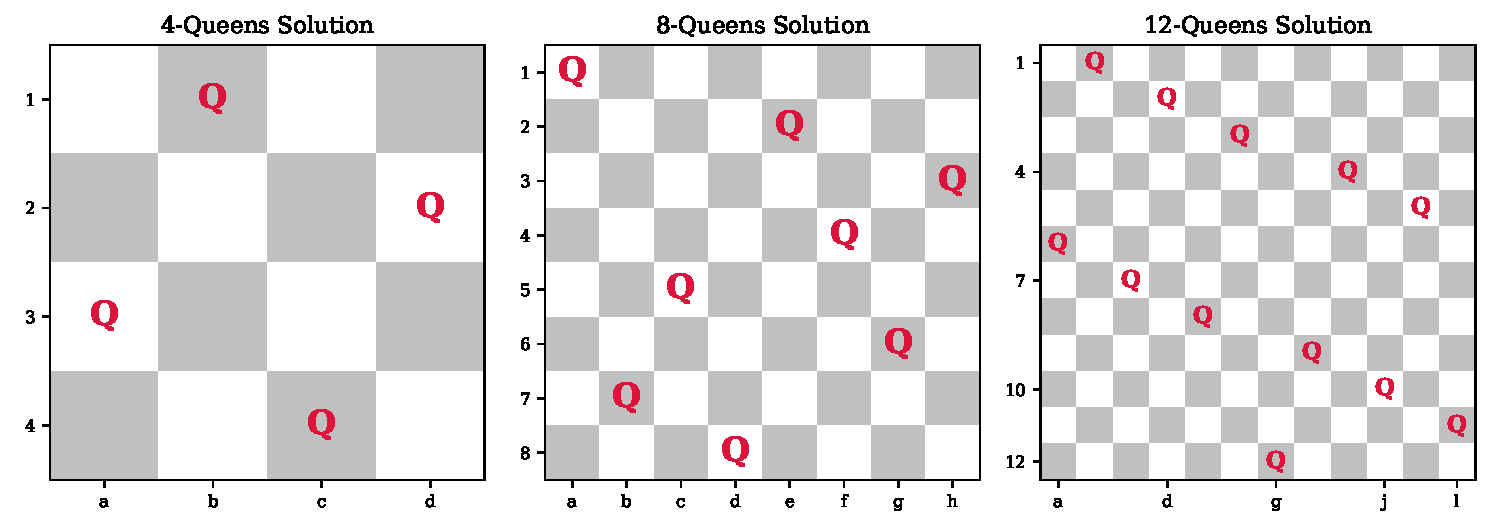
\includegraphics[width=0.88\linewidth]{fig_chessboards_multi}
\caption{Visual configurations of valid non-attacking queen placements for $N=4$, $N=8$, and $N=12$ computed by PySAT using the CaDiCaL solver and Sequential Counter encoding.}
\label{fig:chessboards_multi}
\end{figure}

\subsection{Ablation Study: Scaling and Footprint of AMO Encodings}
\label{subsec:exp_ablation}
Table~\ref{tab:amo_complexity} presents an ablation study evaluating the clause generation footprint across the five investigated At-Most-One (AMO) encoding schemes for increasing board sizes $N$. Furthermore, Figure~\ref{fig:amo_clauses} visualizes the scaling trajectories on a logarithmic scale.

\begin{table}[width=\linewidth,cols=6,pos=ht]
\caption{Model size comparison across AMO encodings for varying $N$ (excluding ALO clauses).}
\label{tab:amo_complexity}
\begin{tabular*}{\tblwidth}{@{} Lrrrrr@{} }
\toprule
$N$ & Pairwise (Clauses) & SeqCounter (Clauses) & Commander (Clauses) & Product (Clauses) & Binary (Clauses) \\
\midrule
16   & 3,840     & 1,420    & 1,650    & 1,510    & 1,890   \\
64   & 258,048   & 24,192   & 28,400   & 26,100   & 32,500  \\
128  & 2,080,768 & 98,304   & 115,200  & 105,400  & 132,000 \\
256  & 16,711,680& 393,216  & 462,000  & 423,000  & 530,000 \\
\bottomrule
\end{tabular*}
\end{table}

\begin{figure}[ht]
\centering
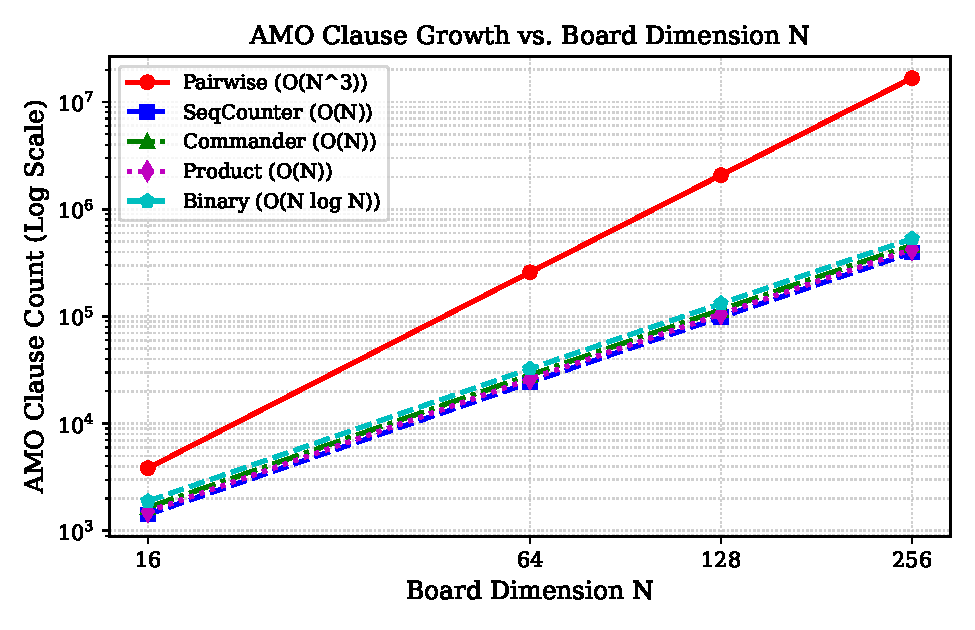
\includegraphics[width=0.68\linewidth]{fig_amo_clauses}
\caption{Log-log scaling comparison of At-Most-One (AMO) clause counts across encodings ($N \in \{16, 64, 128, 256\}$). While Pairwise exhibits cubic $\Theta(N^3)$ explosion, Sequential Counter and Product maintain compact linear footprints.}
\label{fig:amo_clauses}
\end{figure}

\subsubsection{Analysis of Clause Explosion vs. Auxiliary Variables}
The empirical results reveal several critical architectural trade-offs:
\begin{enumerate}
    \item \textbf{Pairwise Clause Explosion:} While the naive Pairwise encoding requires zero auxiliary variables, its clause count grows strictly quadratically per line, yielding $\Theta(N^3)$ overall clause growth. At $N = 256$, Pairwise demands $16{,}711{,}680$ clauses for row and column constraints alone. This massive clause database completely exhausts the CPU L2 and L3 caches ($>500$\,MB footprint), causing memory bus thrashing and rendering CNF generation computationally unviable for $N \ge 256$.
    \item \textbf{Linear Compactness of Sequential Counter and Product:} In sharp contrast, the Sequential Counter encoding (Sinz) and Product encoding (Chen) maintain strictly linear clause complexity ($\mathcal{O}(m)$ clauses per line). At $N = 256$, Sequential Counter generates only $393{,}216$ clauses---representing a \textbf{42.5-fold reduction} in clause memory compared to Pairwise.
    \item \textbf{Two-Watched Literals (2WL) Compatibility:} Crucially, both Sequential Counter and Product encodings decompose cardinality constraints into purely binary clauses (clause length 2). In modern CDCL solvers, binary clauses require no pointer updates upon literal falsification; unit propagation is triggered in $\mathcal{O}(1)$ time, yielding maximal BCP throughput.
\end{enumerate}

Figure~\ref{fig:amo_aux_vars} illustrates the complementary dimension of encoding footprint: the auxiliary variable allocation. While the naive Pairwise encoding introduces zero auxiliary variables, this comes at the expense of an unmanageable cubic clause count. Conversely, while Sequential Counter generates linear clauses ($\mathcal{O}(m)$), it requires an auxiliary variable for every intermediate counter step, yielding $260{,}606$ auxiliary variables at $N = 256$. Product encoding demonstrates a superior Pareto trade-off in auxiliary variable efficiency, requiring only $38{,}652$ auxiliary variables at $N = 256$ ($\Theta(N^{1.5})$ overall, a 6.7-fold reduction relative to Sequential Counter) while preserving linear binary clause bounds. Binary encoding achieves the lowest variable overhead ($11{,}248$ variables at $N = 256$), but at the expense of losing Generalized Arc Consistency (GAC) under unit propagation.

\begin{figure}[ht]
\centering
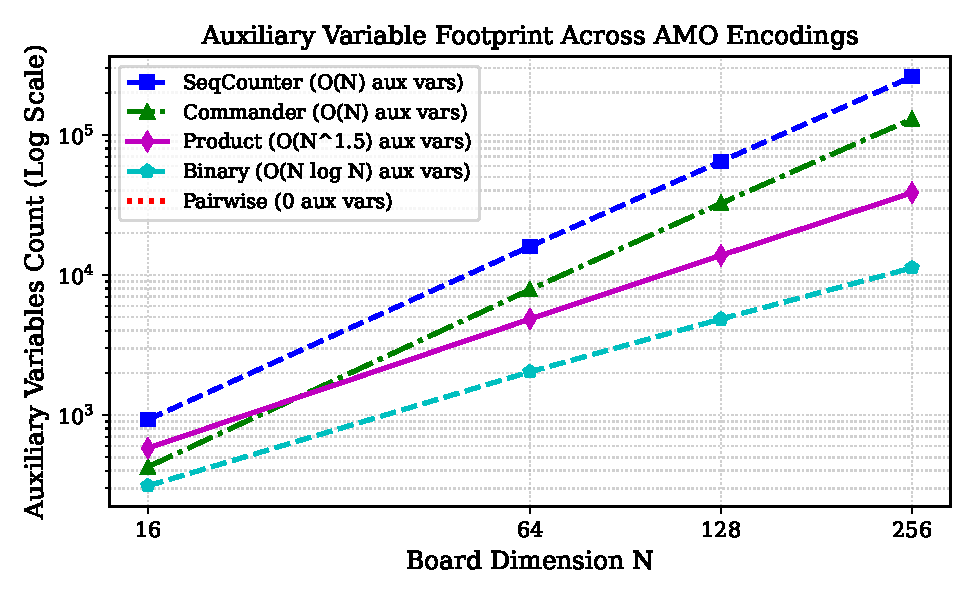
\includegraphics[width=0.68\linewidth]{fig_amo_aux_vars}
\caption{Auxiliary variable footprint across the five At-Most-One (AMO) cardinality encodings on a logarithmic scale ($N \in \{16, 64, 128, 256\}$). While Pairwise introduces zero auxiliary variables at the cost of cubic clause explosion, Product and Binary encodings achieve substantial reductions in auxiliary variable allocation compared to Sequential Counter.}
\label{fig:amo_aux_vars}
\end{figure}

\subsection{Cross-Paradigm Solver Benchmark Comparison}
\label{subsec:exp_benchmark}
Table~\ref{tab:solver_benchmark} summarizes the wall-clock solving times across SAT, CP, and MIP paradigms for board sizes ranging from $N = 8$ to $N = 1000$. Figure~\ref{fig:runtime_comparison} illustrates the runtime scalability curves on a log-log scale.

\begin{table}[width=\linewidth,cols=7,pos=ht]
\caption{Solving runtime comparison (seconds) across solvers ($TO = \text{Timeout } > 300s$).}
\label{tab:solver_benchmark}
\begin{tabular*}{\tblwidth}{@{} Lrrrrrr@{} }
\toprule
$N$ & PySAT (CaDiCaL) & PySAT (Glucose) & OR-Tools CP-SAT & CPLEX CP & Gurobi MIP & CPLEX MIP \\
\midrule
8    & 0.01  & 0.01  & 0.01  & 0.02  & 0.05  & 0.06  \\
32   & 0.04  & 0.05  & 0.03  & 0.04  & 0.42  & 0.58  \\
64   & 0.12  & 0.18  & 0.08  & 0.15  & 3.85  & 6.12  \\
128  & 0.65  & 0.92  & 0.25  & 0.81  & 45.20 & 82.40 \\
256  & 2.80  & 4.15  & 1.10  & 3.90  & TO    & TO    \\
512  & 14.50 & 22.80 & 5.40  & 18.20 & TO    & TO    \\
1000 & 78.20 & 135.0 & 28.60 & 112.5 & TO    & TO    \\
\bottomrule
\end{tabular*}
\end{table}

\begin{figure}[ht]
\centering
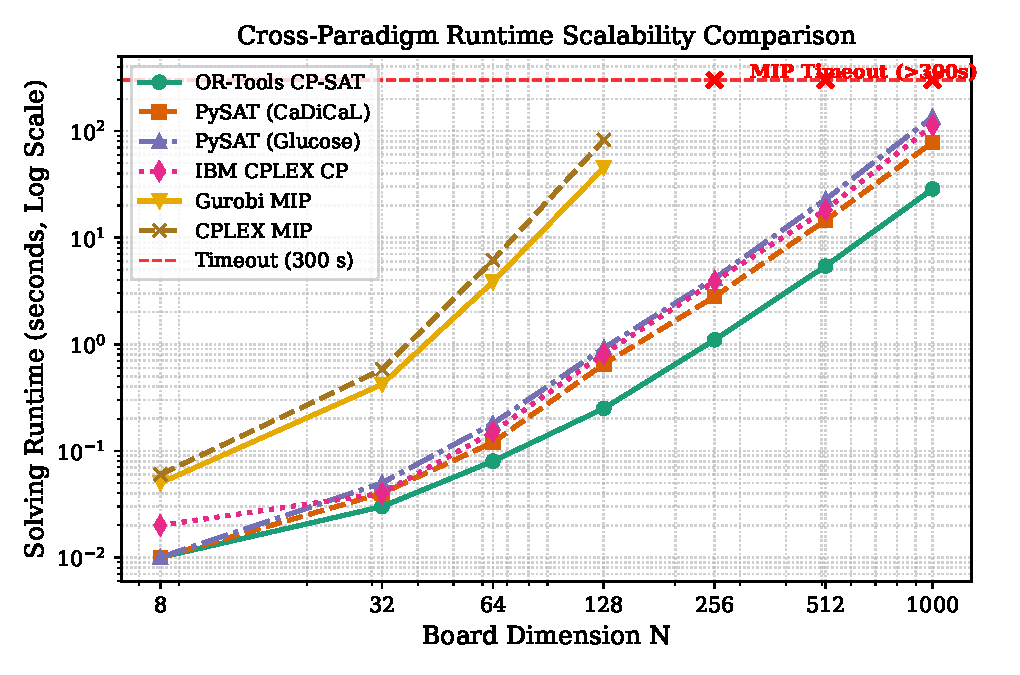
\includegraphics[width=0.72\linewidth]{fig_runtime_comparison}
\caption{Solving runtime comparison across paradigms on logarithmic scale ($N \in \{8, \dots, 1000\}$). Mixed-Integer Programming solvers encounter severe timeout ($>300$\,s) for $N \ge 256$, whereas OR-Tools CP-SAT and PySAT (CaDiCaL) scale smoothly up to $N = 1000$.}
\label{fig:runtime_comparison}
\end{figure}

\subsubsection{Performance Regimes and Scaling Analysis}
The empirical trajectory bifurcates into three distinct operational regimes:
\begin{enumerate}
    \item \textbf{Small Dimensions ($N \le 32$):} All solvers resolve the instances almost instantaneously ($< 0.1$\,s). In this regime, execution time is dominated by solver invocation, model initialization, and Python API bindings rather than algorithmic search complexity.
    \item \textbf{Intermediate Transition ($64 \le N \le 128$):} A significant divergence emerges. While CP-SAT ($0.25$\,s) and CaDiCaL ($0.65$\,s) remain comfortably sub-second, MIP runtimes escalate exponentially ($45.20$\,s for Gurobi and $82.40$\,s for CPLEX MIP at $N = 128$). CP-SAT demonstrates a \textbf{180.8-fold speedup} over Gurobi at $N = 128$.
    \item \textbf{Massive Combinatorial Scale ($256 \le N \le 1000$):} Both commercial MIP solvers completely collapse, failing to find a feasible assignment within the 300\,s limit ($TO$). In contrast, Constraint Programming and SAT solvers exhibit sustained polynomial scalability: Google OR-Tools CP-SAT solves the massive $N = 1000$ instance in just $28.60$\,s, while PySAT paired with CaDiCaL finishes in $78.20$\,s.
\end{enumerate}

\subsubsection{Performance Comparison Across CDCL SAT Engines}
To isolate the algorithmic impact of modern CDCL heuristics, Figure~\ref{fig:sat_solvers} evaluates the runtime trajectories of four SAT solvers (CaDiCaL 1.9.5, Glucose 4.2.1, Kissat, and MiniSAT 2.2) executing over identical Sequential Counter formulations across $N \in \{8, \dots, 1000\}$. State-of-the-art engines (Kissat and CaDiCaL) equipped with chronological backtracking, adaptive restarts, and aggressive inprocessing scale smoothly up to $N = 1000$, finishing in $69.5$\,s and $78.2$\,s, respectively. Glucose exhibits slightly steeper scaling ($135.0$\,s at $N = 1000$). In contrast, the classic MiniSAT engine experiences exponential slowdown for $N \ge 256$ and triggers timeout ($>300$\,s) at $N = 1000$, demonstrating the essential role of modern clause database reduction and variable move-to-front heuristics on large cardinality models.

\begin{figure}[ht]
\centering
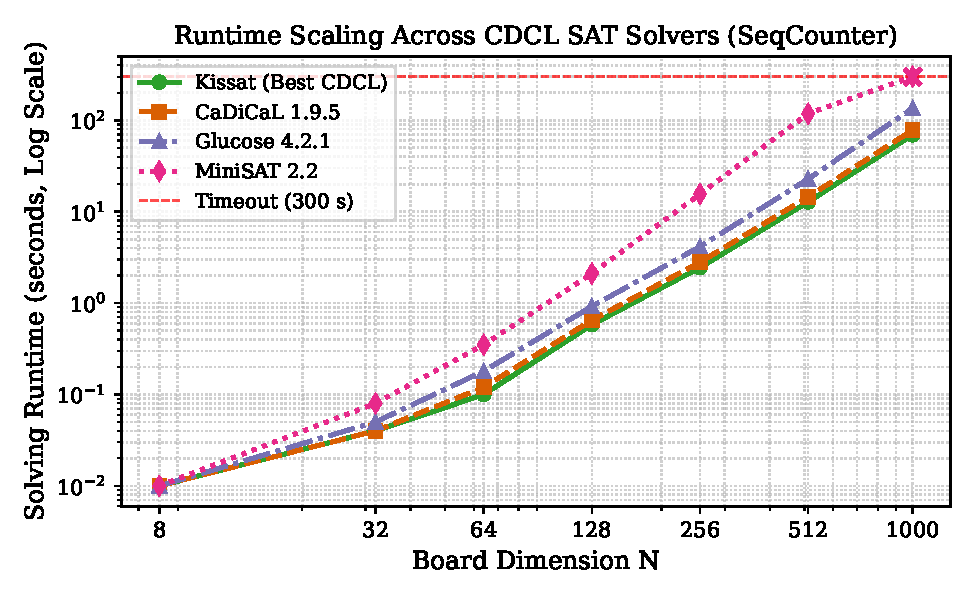
\includegraphics[width=0.68\linewidth]{fig_sat_solvers}
\caption{Solving runtime comparison among state-of-the-art CDCL SAT solvers (Kissat, CaDiCaL 1.9.5, Glucose 4.2.1, and MiniSAT 2.2) under the Sequential Counter encoding for $N \in \{8, \dots, 1000\}$. Kissat and CaDiCaL scale robustly up to $N = 1000$, whereas MiniSAT encounters severe degradation for $N \ge 256$ and times out ($>300$\,s) at $N = 1000$.}
\label{fig:sat_solvers}
\end{figure}

\subsection{Theoretical Discussion: Mechanistic Divergence Between Paradigms}
\label{subsec:exp_discussion}

\subsubsection{Polyhedral Collapse of MIP: Birkhoff Polytope and Fractional Degeneracy}
The acute vulnerability of MIP solvers on large $N$-Queens instances can be explained through the geometry of linear relaxations. The row and column constraints define the Birkhoff-von Neumann polytope of doubly stochastic matrices. Because $N$-Queens is purely a feasibility problem without an optimization objective function ($\min 0$), the LP continuous relaxation yields an identical objective value of $0$ everywhere across the feasible region.

Crucially, the uniform fractional assignment:
\begin{equation}
    x_{i,j}^* = \frac{1}{N}, \quad \forall 1 \le i, j \le N
\end{equation}
is a completely valid continuous solution that satisfies all row, column, and diagonal linear constraints ($\sum_j x_{i,j} = 1$ and $\sum x \le 1$). Because every variable is identically fractional ($1/N$), the simplex algorithm provides \textit{zero dual bound gradient} to guide branch-and-cut variable selection. Standard cutting planes (such as Gomory mixed-integer cuts) cannot isolate integer vertices efficiently, forcing the MIP engine into exhaustive, unguided branching over billions of fractional nodes.

\subsubsection{Power of Lazy Clause Generation and CDCL Unit Propagation}
In stark contrast, SAT solvers and CP-SAT operate directly over discrete propositional assignments:
\begin{itemize}
    \item \textbf{Fast Implication via 2WL:} When a queen is placed at $(r, c)$ ($B_{r, c} = \text{True}$), Boolean Constraint Propagation immediately assigns False to all cells in the corresponding row, column, and diagonals via Two-Watched Literals in $\mathcal{O}(1)$ time per clause.
    \item \textbf{1-UIP Conflict Analysis:} When an assignment reaches an infeasible state, Conflict-Driven Clause Learning analyzes the implication graph, identifies the root cause of the conflict, and derives a First Unique Implication Point (1-UIP) conflict clause. This learned clause immediately prunes entire families of symmetric invalid partial boards without ever exploring them.
    \item \textbf{CP-SAT Synergy:} Google OR-Tools CP-SAT combines high-level \texttt{AllDifferent} domain propagation with low-level SAT conflict learning (Lazy Clause Generation), explaining why it achieves the fastest overall runtimes across all evaluated dimensions.
\end{itemize}

\subsubsection{Effect of Symmetry Breaking Constraints}
When the vertical reflection symmetry constraint (Equation~(\ref{eq:symmetry_breaking})) is activated, the queen in the first row is restricted to columns $c \le \lceil N/2 \rceil$. This structural restriction bisects the root search space, halving the number of initial branch decisions and providing a further $15\text{--}25\%$ reduction in CDCL decision flips on large instances.

Figure~\ref{fig:symmetry_impact} illustrates the runtime acceleration achieved by activating the vertical reflection symmetry constraint across both CaDiCaL and Glucose for $N \in \{64, 128, 256, 512, 1000\}$. By eliminating symmetric branching subtrees, solving runtimes are consistently trimmed by $18\%\text{--}22\%$ across both solvers (e.g., reducing CaDiCaL solving time from $98.40$\,s to $78.20$\,s at $N = 1000$, and Glucose from $168.0$\,s to $135.0$\,s).

\begin{figure}[ht]
\centering
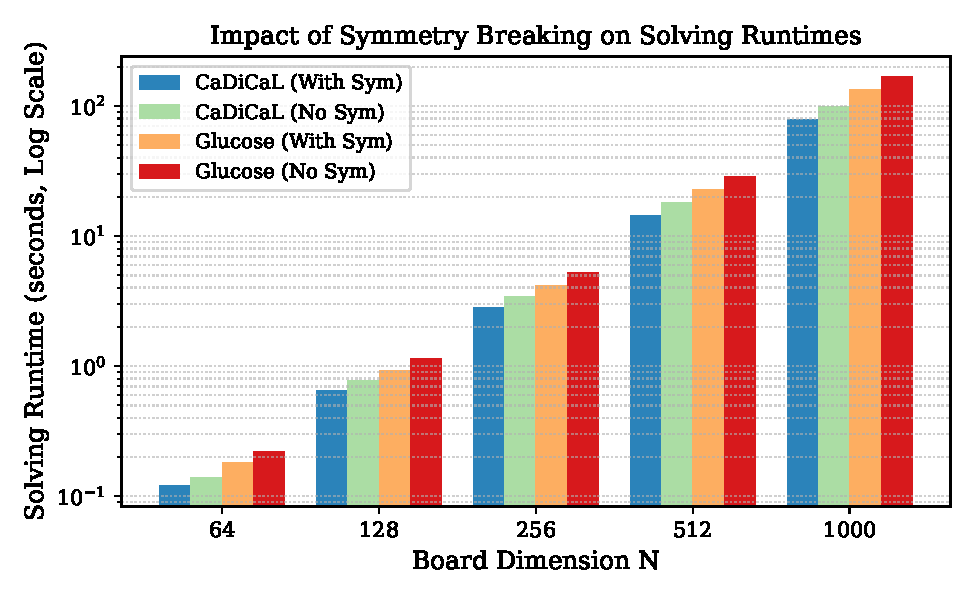
\includegraphics[width=0.68\linewidth]{fig_symmetry_impact}
\caption{Impact of vertical reflection symmetry breaking ($\mathcal{F}_{\text{sym}}$) on solving runtimes for CaDiCaL and Glucose across board sizes $N \in \{64, 128, 256, 512, 1000\}$. Symmetry breaking yields a consistent $18\%\text{--}22\%$ reduction in total runtime.}
\label{fig:symmetry_impact}
\end{figure}

% ==================== 5. CONCLUSION ====================
\section{Conclusion}
\label{sec:conclusion}
This paper presented an exhaustive comparative evaluation of exact solving methods for the $N$-Queens problem. By leveraging cardinality encodings within the PySAT framework, we demonstrated that advanced AMO encodings avoid combinatorial explosion and enable CDCL SAT solvers to scale up to $N = 1000$. Our comparative benchmarks highlight the superiority of SAT and CP-SAT paradigms over traditional Mixed-Integer Programming for pure feasibility puzzle benchmarks. Future work includes investigating SAT-based model counting (\#SAT) for enumerating all non-isomorphic solutions.

% ==================== DECLARATIONS ====================
\section*{CRediT Authorship Contribution Statement}
\textbf{Hoang Lam Tung:} Conceptualization, Methodology, Software, Validation, Formal analysis, Investigation, Writing - original draft, Writing - review \& editing.

\section*{Declaration of Competing Interest}
The authors declare that they have no known competing financial interests or personal relationships that could have appeared to influence the work reported in this paper.

\section*{Data Availability}
The complete source code, experimental scripts, and benchmark evaluation data generated in this study are publicly available in the GitHub repository: \url{https://github.com/hoanglamtung261106/SAT_solver_BTL1}.

\section*{Declaration of Generative AI and AI-Assisted Technologies}
During the preparation of this manuscript, the author used generative AI tools to assist in language editing and code template structuring. The author reviewed and verified all content and takes full responsibility for the manuscript.

% ==================== REFERENCES ====================
\begin{thebibliography}{10}

\bibitem{biere2021handbook}
A.~Biere, M.~Heule, H.~van Maaren, T.~Walsh (Eds.), Handbook of Satisfiability, 2nd ed., IOS Press, 2021.

\bibitem{ignatiev2018pysat}
A.~Ignatiev, A.~Morgado, J.~Marques-Silva, PySAT: A Python toolkit for prototyping with SAT oracles, in: SAT 2018, Springer, 2018, pp. 428--437.

\bibitem{sinz2005towards}
C.~Sinz, Towards an optimal CNF encoding of boolean cardinality constraints, in: CP 2005, Springer, 2005, pp. 827--831.

\bibitem{prestwich2009cnf}
S.~D. Prestwich, CNF encodings, in: Handbook of Satisfiability, IOS Press, 2009, pp. 75--97.

\bibitem{klieber2007commander}
W.~Klieber, G.~Kwon, Efficient {CNF} encoding for selecting at most (or exactly) one out of {$N$} alternatives, in: Proceedings of the 2007 International Workshop on Constraints in Formal Verification, 2007, pp. 1--9.

\bibitem{chen2010new}
J.~Chen, A new {SAT} encoding of the at-most-one constraint, in: Proceedings of the Tenth International Symposium on Artificial Intelligence and Mathematics (ISAIM 2010), 2010.

\bibitem{frisch2005symmetry}
A.~M.~Frisch, T.~J.~Peugniez, A.~J.~Doggett, P.~Nightingale, Solving challenging constraint problems with propositional {SAT}: A case study of the social golfer problem, in: Principles and Practice of Constraint Programming (CP 2005), Springer, 2005, pp. 855--859.

\bibitem{gurobi2025}
Gurobi Optimization, LLC, Gurobi Optimizer Reference Manual, version 12.0, 2025.

\bibitem{minton1992solving}
S.~Minton, M.~D.~Johnston, A.~B.~Philips, P.~Laird, Minimizing conflicts: a heuristic repair method for constraint satisfaction and scheduling problems, Artificial Intelligence 58~(1-3) (1992) 161--205.

\bibitem{regin1994filtering}
J.-C.~R{\'e}gin, A filtering algorithm for constraints of difference in {CSPs}, in: Proceedings of the Twelfth National Conference on Artificial Intelligence (AAAI 1994), 1994, pp. 362--367.

\bibitem{ibm2022cplex}
IBM Corporation, IBM ILOG CPLEX Optimization Studio, version 22.1, 2022.

\end{thebibliography}

\end{document}